\documentclass[11pt]{article}

\usepackage{times}
\usepackage{epsf}
\usepackage{epsfig}
\usepackage{amsmath, alltt, amssymb, xspace}
\usepackage{wrapfig}
\usepackage{fancyhdr}
\usepackage{url}
\usepackage{verbatim}
\usepackage{fancyvrb}
\usepackage{float}

\usepackage{subfigure}
\usepackage{cite}
\usepackage{hyperref}
\hypersetup{%
    pdfborder = {0 0 0}
}
\topmargin      -0.50in  % distance to headers
\oddsidemargin  0.0in
\evensidemargin 0.0in
\textwidth      6.5in
\textheight     8.9in 


%\centerfigcaptionstrue

%\def\baselinestretch{0.95}


\newcommand\discuss[1]{\{\textbf{Discuss:} \textit{#1}\}}
%\newcommand\todo[1]{\vspace{0.1in}\{\textbf{Todo:} \textit{#1}\}\vspace{0.1in}}
\newtheorem{problem}{Problem}[section]
%\newtheorem{theorem}{Theorem}
%\newtheorem{fact}{Fact}
\newtheorem{define}{Definition}[section]
%\newtheorem{analysis}{Analysis}
\newcommand\vspacenoindent{\vspace{0.1in} \noindent}

%\newenvironment{proof}{\noindent {\bf Proof}.}{\hspace*{\fill}~\mbox{\rule[0pt]{1.3ex}{1.3ex}}}
%\newcommand\todo[1]{\vspace{0.1in}\{\textbf{Todo:} \textit{#1}\}\vspace{0.1in}}

%\newcommand\reducespace{\vspace{-0.1in}}
% reduce the space between lines
%\def\baselinestretch{0.95}

\newcommand{\fixmefn}[1]{ \footnote{\sf\ \ \fbox{FIXME} #1} }
\newcommand{\todo}[1]{
\vspace{0.1in}
\fbox{\parbox{6in}{TODO: #1}}
\vspace{0.1in}
}

\newcommand{\mybox}[1]{
\vspace{0.2in}
\noindent
\fbox{\parbox{6.5in}{#1}}
\vspace{0.1in}
}


\newcounter{question}
\setcounter{question}{1}

\newcommand{\myquestion} {{\vspace{0.1in} \noindent \bf Question \arabic{question}:} \addtocounter{question}{1} \,}

\newcommand{\myproblem} {{\noindent \bf Problem \arabic{question}:} \addtocounter{question}{1} \,}


\newcommand{\copyrightnotice}[1]{
\vspace{0.1in}
\fbox{\parbox{6in}{
      This lab was developed for the Labtainer framework by the Naval Postgraduate
      School, Center for Cybersecurity and Cyber Operations under sponsorship from
      the DoD CySP program.  This work is in the public domain, and cannot be copyrighted.}}
\vspace{0.1in}
}


\newcommand{\idea}[1]{
\vspace{0.1in}
{\sf IDEA:\ \ \fbox{\parbox{5in}{#1}}}
\vspace{0.1in}
}

\newcommand{\questionblock}[1]{
\vspace{0.1in}
\fbox{\parbox{6in}{#1}}
\vspace{0.1in}
}


\newcommand{\argmax}[1]{
\begin{minipage}[t]{1.25cm}\parskip-1ex\begin{center}
argmax
#1
\end{center}\end{minipage}
\;
}

\newcommand{\bm}{\boldmath}
\newcommand  {\bx}    {\mbox{\boldmath $x$}}
\newcommand  {\by}    {\mbox{\boldmath $y$}}
\newcommand  {\br}    {\mbox{\boldmath $r$}}


\newcommand{\tstamp}{\today}   
%\rfoot[\fancyplain{\tstamp} {\tstamp}]  {\fancyplain{}{}}

\pagestyle{fancy}
\lhead{\bfseries Labtainers}
\chead{}
\rhead{\small \thepage}
\lfoot{}
\cfoot{}
\rfoot{}




\begin{document}

\begin{center}
{\LARGE ARP Spoofing for Sniffing and Man-in-the-middle Attacks}
\vspace{0.1in}\\
\end{center}

\copyrightnotice

\section{Overview}
This exercise explores the use of ARP spoofing as a means to
sniff local network traffic.  Modern Local Area Networks (LANs)
use ethernet switches, which prevent passive sniffing of network
traffic between other components.  This lab assumes you have
separately learned about the ARP protocol.  ARP spoofing is
a technique by which the attacker sends spoofed ARP messages
into the LAN, with a goal of causing traffic meant for one IP
address to be routed to the attacker's computer instead.  The
attacker's computer then forwards the traffic to the intended
destination.  This puts the attacker into the middle of the
traffic exchange, hence the name "Man in the Middle" attack.

\section{Lab Environmnet}
This lab runs in the Labtainer framework,
available at http://nps.edu/web/c3o/labtainers.
That site includes links to a pre-built virtual machine
that has Labtainers installed, however Labtainers can
be run on any Linux host that supports Docker containers.

From your labtainer-student directory start the lab using:
\begin{verbatim}
    labtainer arp-spoof
\end{verbatim}
Links to this lab manual and to an empty lab report will be displayed.  If you create your lab report on a separate system, 
be sure to copy it back to the specified location on your Linux system.


\section{Network Configuration}
This lab includes four networked computers as shown in Figure~\ref{fig:intended},
which illustrates the intended flow of traffic between the user computer and
the Webserver via the Gateway.  

\begin{figure}[H]
\begin{center}
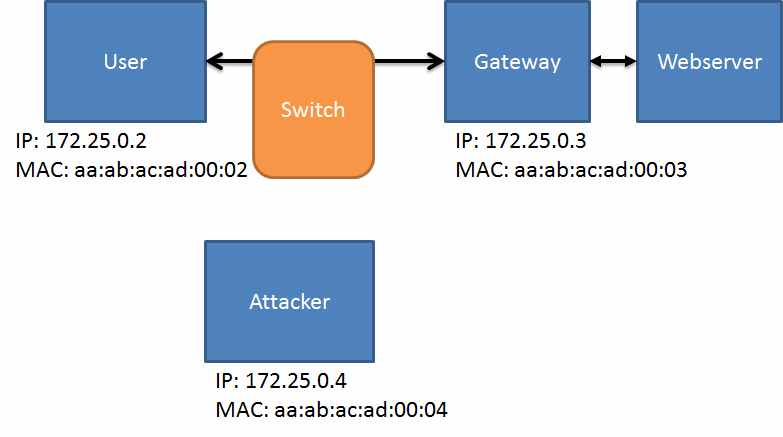
\includegraphics [width=0.8\textwidth]{figure1.jpg}
\end{center}
\caption{Intended traffic from between User and Webserver}
\label{fig:intended}
\end{figure}

\section{Lab Tasks}
In this lab, you will use the {\tt arpspoof} tool to convice the User computer that
traffic destined for Gateway should instead be sent to the Attacker computer -- and
convince the Gateway that traffic destined for the User should be sent to the Attacker
computer, as illustrated in ~Figure\ref{fig:spoofed}
\begin{figure}[H]
\begin{center}
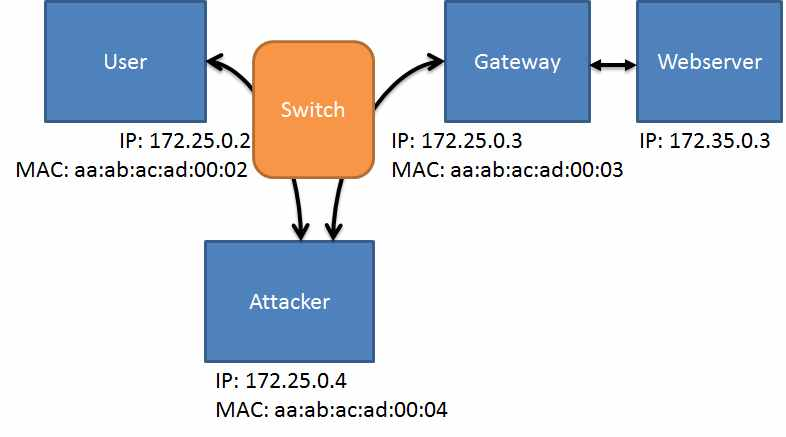
\includegraphics [width=0.8\textwidth]{figure2.jpg}
\end{center}
\caption{Man-in-the-middle attack via ARP Spoofing}
\label{fig:spoofed}
\end{figure}

The {\tt arpspoof} tool is installed on the Attacker computer, as is Wireshark.
The Attacker computer is configured to forward IP packets that is receives which
are destined for elsewhere.  You can confirm this with this command, which should
reflect a value of '1':
\begin{verbatim}
   sysctl net.ipv4.conf.all.forwarding
\end{verbatim}

\subsection{Task 1: Sniff the LAN from the Attacker}
Before you engage in ARP spoofing, first look at network traffic as seen by
the Attacker.
Start Wireshark on the Attacker computer, selecting the "eth0" interface:
\begin{verbatim}
   wireshark -ki eth0
\end{verbatim}

On the User computer, use wget to retrieve a web page from the Webserver:
\begin{verbatim}
   wget <address of Webserver>
\end{verbatim}

\noindent Observe the Wireshark display.  Do you see either the web query or the response?

\subsection{Task 2: Spoof the ARP cache on the User and Gateway Computers}
Use the arpspoof tool on the Attacker computer to perform your ARP spoofing.
Note you must target both the User and Gateway computers.  It is easiest to
start the arpspoof program in two different virtual terminals connected to the 
attacker (you may have wondered why you were given three Attacker terminals).

\begin{verbatim}
    sudo arpspoof -t <User IP> <gateway IP>
    sudo arpspoof -t <gateway IP> <User IP>
\end{verbatim}


After your ARP spoofing has commenced you should see your spoofed ARP traffic in Wireshark.
Now return to the User computer and refetch
the web page using {\tt wget} command.  You should see TCP traffic in your Wireshark
display.  In Wireshark, stop the capture, (red button), and use 
"File / Save" to save the traffic into a file named sniff.pcapng in your HOME directory,
(/home/ubuntu).

\section{Submission}
After finishing the lab, go to the terminal on your Linux system that was used to start the lab and type:
\begin{verbatim}
    stoplab arp-spoof
\end{verbatim}
When you stop the lab, the system will display a path to the zipped lab results on your Linux system.  Provide that file to 
your instructor, e.g., via the Sakai site.

\end{document}
